\section{Model2D  Class Reference}
\label{class_Model2D}\index{Model2D@{Model2D}}
Base for all 2D models. 


{\tt \#include $<$model2d.h$>$}

Inheritance diagram for Model2D::\begin{figure}[H]
\begin{center}
\leavevmode
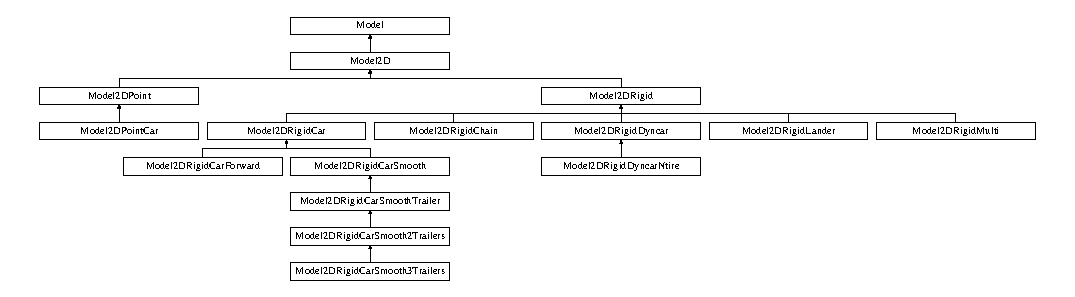
\includegraphics[height=3.5387cm]{class_Model2D}
\end{center}
\end{figure}
\subsection*{Public Methods}
\begin{CompactItemize}
\item 
{\bf Model2D} (string path)
\item 
virtual {\bf $\sim$Model2D} ()
\item 
virtual {\bf MSLVector} {\bf State\-To\-Configuration} (const {\bf MSLVector} \&x)
\begin{CompactList}\small\item\em A method that converts a {\bf Model} {\rm (p.\,\pageref{class_Model})} state in to a {\bf Geom} {\rm (p.\,\pageref{class_Geom})} configuration.\item\end{CompactList}\end{CompactItemize}


\subsection{Detailed Description}
Base for all 2D models.



\subsection{Constructor \& Destructor Documentation}
\index{Model2D@{Model2D}!Model2D@{Model2D}}
\index{Model2D@{Model2D}!Model2D@{Model2D}}
\subsubsection{\setlength{\rightskip}{0pt plus 5cm}Model2D::Model2D (string {\em path})}\label{class_Model2D_a0}


\index{Model2D@{Model2D}!~Model2D@{$\sim$Model2D}}
\index{~Model2D@{$\sim$Model2D}!Model2D@{Model2D}}
\subsubsection{\setlength{\rightskip}{0pt plus 5cm}Model2D::$\sim$Model2D ()\hspace{0.3cm}{\tt  [inline, virtual]}}\label{class_Model2D_a1}




\subsection{Member Function Documentation}
\index{Model2D@{Model2D}!StateToConfiguration@{StateToConfiguration}}
\index{StateToConfiguration@{StateToConfiguration}!Model2D@{Model2D}}
\subsubsection{\setlength{\rightskip}{0pt plus 5cm}virtual {\bf MSLVector} Model2D::State\-To\-Configuration (const {\bf MSLVector} \& {\em x})\hspace{0.3cm}{\tt  [virtual]}}\label{class_Model2D_a2}


A method that converts a {\bf Model} {\rm (p.\,\pageref{class_Model})} state in to a {\bf Geom} {\rm (p.\,\pageref{class_Geom})} configuration.



Reimplemented from {\bf Model} {\rm (p.\,\pageref{class_Model_a8})}.

Reimplemented in {\bf Model2DRigid} {\rm (p.\,\pageref{class_Model2DRigid_a6})}, {\bf Model2DRigid\-Car\-Smooth} {\rm (p.\,\pageref{class_Model2DRigidCarSmooth_a5})}, {\bf Model2DRigid\-Car\-Smooth\-Trailer} {\rm (p.\,\pageref{class_Model2DRigidCarSmoothTrailer_a4})}, {\bf Model2DRigid\-Car\-Smooth2Trailers} {\rm (p.\,\pageref{class_Model2DRigidCarSmooth2Trailers_a4})}, {\bf Model2DRigid\-Car\-Smooth3Trailers} {\rm (p.\,\pageref{class_Model2DRigidCarSmooth3Trailers_a4})}, {\bf Model2DRigid\-Dyncar} {\rm (p.\,\pageref{class_Model2DRigidDyncar_a3})}, {\bf Model2DRigid\-Lander} {\rm (p.\,\pageref{class_Model2DRigidLander_a3})}, {\bf Model2DRigid\-Multi} {\rm (p.\,\pageref{class_Model2DRigidMulti_a3})}, and {\bf Model2DRigid\-Chain} {\rm (p.\,\pageref{class_Model2DRigidChain_a2})}.

The documentation for this class was generated from the following file:\begin{CompactItemize}
\item 
{\bf model2d.h}\end{CompactItemize}
